We have seen in the previous chapter that the encode-decode method can be used
in a variety of cases when we want to make statements about the equality
types -- or \emph{path spaces} -- of higher inductive types.
Going through all necessary steps of such a proof can be somewhat tedious, but
part of it is very mechanical work.
One main goal of this chapter is to present a different method to
directly work with equality types of coequalizers and pushouts
(and constructions based on these):
Since elimination rules such as the one for coequalizers characterize only
the points  of the type, but in the constructors we create points
and equalities simultaneously, we believe that it is natural to hope for
an ``induction principle for equalities'' which is reminiscent of an elimination
rule.
More concretely, for our case of a coequalizer $\quot : \UU$ of a type $A : \UU$
and typal relation $\_\sim\_ : A \to A \to \UU$,
let us assume we are given a type family
\begin{equation*}
Q: \{a, b : A\} \to [a] = [b] \to \UU \text{.}
\end{equation*}
Is it possible to have simple-to-check conditions which are sufficient to
conclude $Q(q)$ for a general $q$ (instead of just $glue(s)$ for some $s : a \sim b$)?

\begin{remark}
Note that $Q$ above quantifies over two elements of $A$ and an equality of $\quot$.
If instead we asked the same question for a type family
\begin{equation*}
S: (x, y : \quot) \to x = y \to \UU \text{,}
\end{equation*}
the answer would be that we could use the J-rule to populate this family by giving
$S(\refl_x)$.
The principle we want for the applications we presented is the version
where endpoints are ``restricted'' as above.
\end{remark}

It turns out that, like for the J-rule, there is a generalization of the above question.
We get this generalization by switching from an \emph{unbased} (or \emph{global}) type family
to a \emph{based} (or \emph{local}) one:
We can fix one of the two endpoints to be $[a_0] : \quot$ and replace $Q$
by a family which is indexed only \emph{once} over $A$:
\begin{equation}
P : (b : A) \to [a_0] = [b] \to \UU \text{.}
\end{equation}
Like for the two versions of the J-rule, a principle answering the based version
of the question also answers the unbased one, which is why we will focus
exclusively on the former, and we will be able to easily derive the latter from it.

In order to get some intuition for the subtleties of the equality types,
let us first look at a hypothetical principle which turns out to be wrong.
Usually, induction principles contain one case for every constructor,
the standard equality constructor is $\refl$ and with \textsc{Coeq-Intro2}, we
have one further path constructor $\glue$.
Thus, we might try whether it is sufficient to assume terms
\begin{align*}
r &: P(a_0, \refl_{[a_0]}) \text{ and}\\
p &: (b : A)(s : a_0 \sim b) \to P(b, \glue(s))
\end{align*}
to conclude that $(b : A)(q : [a_0] = [b]) \to P(b, q)$?
It turns out that this attempt fails:
Consider the relation $\sim$ on the natural numbers defined by
\begin{equation*}
(m \sim n) :\equiv m + 1 = n \text{.}
\end{equation*}
We can look at the coequalizer $\specialquot{\N}$.
Let us take $1 : \N$ as the base point and $P : (n : \N) \to ([0] = [n]) \to \UU$
defined by $P(n,q) :\equiv (n \geq 1)$.
The terms $r$ and $p$ are constructed easily, but at the same time, it is clear
that $P(0, \glue(k)\inv)$ is empty (here, $k$ is a proof for $0 + 1 = 1$).

The above naïve suggestion was easy to disprove, but let us try to understand
why it was insufficient.
Equalities that come from $A$ can, by the J-rule, be assumed to be $\refl$;
these are sufficiently covered.
However this is not true for equalities that are generated using the $\glue$ constructor.
The counterexample uses the fact that we have not explicitely closed them under symmetry
and similarity -- we could have also used that we have not closed them
under transitivity.

How could we fix this? Given an equality $q$ in $\quot$, we can compose it
with $\glue(s)$ assuming the endpoints match.
This suggests that the induction principle we are looking for should assume
$Q(q) \to Q(q \ct \glue(s))$.
But we can also compose with $\glue(s)\inv$,
suggesting that we also need a function $Q(q)  \to Q(q \ct \glue(s)\inv)$.
The operations of composing with $\glue(s)$ and its inverse should furthermore
be inverse to each other,
wich motivates us to ask for only \emph{one} of them and require this one to be
an equivalence, i.\,e. $Q(q) \simeq Q(q \ct \glue(s))$.
This finally leads us to a valid induction principle, which is short, useful, and
comes with two $\beta$-rules.
Proving this princple is the main result of this chapter:

%\begin{restatable}[Induction for Coequalizer Equality]{thm}{main-thm}
\begin{thm}[Induction for Coequalizer Equality]\label{thm:paths-main-thm}
Assume $A$ and $\sim$ as before, a point $a_0 : A$, and we are further given
a type family
\begin{equation*}
P : (b : A) \to [a_0] = [b] \to \UU \text{,}
\end{equation*}
together with terms
\begin{align*}
r &: P(\refl_{[a_0]}) \text{ and} \\
e &: \{b, c : A\}(q : [a_0] = [b])(s : b \sim c) \to P(q) \simeq P(q \ct \glue(s)) \text{.}
\end{align*}
The we can construct a dependent function
\begin{equation*}
\ind_{r, e} : \{b : A\}(q : [a_0] = [b]) \to P(q)
\end{equation*}
with the following equalities reminiscent of $\beta$-rules:
\begin{align}
\ind_{r,e} (\refl_{[a_0]}) &= r \label{eq:paths-thm-based-first-beta} \\
\ind_{r,e}(q \ct \glue(s)) &= e (q,s, \mathsf{ind}_{r,e}(q)) \label{eq:paths-thm-based-second-beta} \text{.}
\end{align}
\end{thm}

\begin{remark}
The theorem can be proved in a way which makes the first $\beta$-rule hold judgmentally.
This is what we have done in our formalization, but we will refrain from checking
whether equalities hold strictly in this chapter.
\end{remark}

In the following sections we will first prove this main result (Chapter~\ref{sec:paths-main}),
then modify it to obtain a version for pushouts (Chapter~\ref{sec:paths-pushout}),
and present a few smaller applications (Chapter~\ref{sec:paths-applications})
by characterizing the loop space of the circle and proving that
pushouts preserve embeddings,
before applying the approach to state a version of the Seifert-van Kampen theorem
which instead of groupoids refers to \emph{higher} fundamental groupoids
(Chapter~\ref{sec:paths-svk}).
Most of the contents have been formalized in Lean, an effort which we will
comment on in Chapter~\ref{sec:paths-lean}.

\section{The Main Theorem: Path Spaces in Coequalizers}\label{sec:paths-main}

We will first formulate and prove the non-dependent version of the main result
by developing the corresponding categorical framework inside type theory.
This then allows us to derive the induction principle as stated in Theorem~\ref{thm:paths-main-thm}.

Using categorical ideas to structure constructions and reason inside type
theory is standard.
The dependent elimination principle can usually equivalently be formulated
as a recursion (or \emph{non-dependent} elimination) principle together
with a uniqueness principle,
often phrased as a \emph{universal property}.
A principled way of doing this is to define objects and morphisms of a
category; the statement then is that the inductive type in question is
(homotopy) initial in this category.
For the specific case of homotopy type theory, the connection between
induction and initiality has been shown by
\cite{awodeyGamSoja_hoAlgs} for inductive types,
and by \cite{DBLP:journals/corr/Sojakova14} for some higher inductive types.

However, category theory in homotopy type theory is subtle.
The ``obvious'' naïve definition of a category without imposing any
truncation levels on objects and morphisms (sometimes called a
\emph{wild category}) is not always a well-behaved notion.
For example the slice of a wild category is not a wild category anymore.
The underlying reason is that the identity and associativity
equalities do not behave like laws (or properties) but like higher morphisms
in a \emph{higher category} where additional coherences are required.
One approach to higher categories in homotopy type theory
is discussed by~\cite{Capriotti2017}.
Alternatively, the \emph{univalent categories} by~\cite{ahrens_rezk}
restrict the truncation levels to avoid the issue.
For us,
truncating is not a suitable strategy since it would not allow us to prove our general result.

Although not well-behaved in general, wild categories are still a useful tool
for us.
We do \emph{not} think of them as ``bad ordinary categories'' but instead
as an approximation to $(\infty,1)$-categories, where most of the
higher data is omitted.
However, since none of our constructions require us to actually \emph{use}
the omitted data, we are able to get away with this.
Most importantly,
we can talk about the concept of homotopy initiality without ever referring
to higher morphisms.
Technically, we do not even need associativity -- it could be excluded from the
following definition without consequences for the rest of the section.

\begin{defn}[Wild Categories]
A \textbf{wild category} $\CatA$, for simplicity henceforth simply
\textbf{category}, consists of a type $\bproj{\CatA} : \UU$ of objects; for
objects $X, Y : \bproj \CatA$ a type $\CatA(X, Y)$ of morphisms;
a composition operator $\circ$ and identities of the following obvious types
\begin{align*}
\_\circ\_ &: \{X, Y, Z : \bproj \CatA\} \to \CatA(Y, Z) \to \CatA(X, Y) \to \CatA(X, Z) \text{,} \\
\id &: \{X : \bproj \CatA\} \to \CatA(X, X) \text{,}
\end{align*}
together with the two standard equalities for the identities and
one equality which states that $\circ$ is associative:
\begin{align*}
\id \circ f &= f \text{,}\\
f \circ \id &= f \text{, and}\\
(f \circ g) \circ h &= f \circ (g \circ h) \text{.}
\end{align*}
\end{defn}

Initiality is one of the few notions which are still well-behaved
in wild categories:
We can define it in terms of contractability.
\begin{defn}[Initiality]
An object $X$ of a category $\CatA$ is called \textbf{initial} if for every
object $Y$ the type of morphisms $\CatA(X, Y)$ is contractible.
\end{defn}

For the whole remainder of the section, let us assume that a type $A : \UU$
together with a point $a_0 : A$ and a relation $\_\sim\_ : A \to A \to \UU$ are
given.
Our main category of interest is the following:

\begin{defn}[Category of Coherent, Pointed Families]\label{def:paths-catC}
The category $\CatC$ is defined as follows:
Objects in $\bproj \CatC$ are ``pointed type families respecting $\sim$'',
by which we mean triples $(K, r, e)$ of the types
\begin{align*}
K &: A \to \UU \text{,} \\
r &: K(a_0) \text{, and} \\
e &: \{b, c : A\}(b \sim c) \to K(b) \simeq K(c) \text{.}
\end{align*}
Morphisms are ``pointed fibrewise functions''.
Explicitely, a morphism in $\CatC((K, r, e), (K', r', e'))$ is 
a triple $(f, \gamma, \delta)$ with
\begin{align*}
f &: (b : A) \to K(b) \to K'(b) \text{,} \\
\gamma &: f_{a_0}(r) = r' \text{, and} \\
\delta &: \{b, c : A\}(s : b \sim c) \to e'(s) \circ f_b = f_c \circ e(s) \text{.}
\end{align*}
It might be helpful to think of $\gamma$ as an equality witnessing that, for any
$s : b \sim c$ the following square commutes:
 \begin{equation} \label{eq:commuting-square}
  \begin{tikzpicture}[x=\diagx,y=-\diagy,baseline=(current bounding box.center)]
   \node (Kab) at (0,0) {$K(b)$};
   \node (Kac) at (1,0) {$K(c)$};
   \node (Kpab) at (0,1) {$K'(b)$};
   \node (Kpac) at (1,1) {$K'(c)$};
  
   \draw[->] (Kab) to node [above] {$\scriptstyle e(s)$} (Kac);
   \draw[->] (Kpab) to node [above] {$\scriptstyle e'(s)$} (Kpac);
   \draw[->] (Kab) to node [left] {$\scriptstyle f_b$} (Kpab);
   \draw[->] (Kac) to node [right] {$\scriptstyle f_c$} (Kpac);
  \end{tikzpicture}
 \end{equation}
The remaining components (identities, composition and their equations) are
straightforward to define.
For example identities are given as
\begin{equation*}
(\lambda b.\, \id, \refl_{r}, \lambda s.\, \refl_{e(s)}) \text{,}
\end{equation*}
and composition is given by
\begin{equation*}
(f', \delta', \gamma') \circ (f, \delta, \gamma)
  :\equiv (\lambda b. ({f_b}' \circ f_b), \ap_{f'_{a_0}}(\delta) \ct \delta', \gamma' \circ \gamma) \text{,}
\end{equation*}
where the last bit is given by pasting two vertically neighboring
squares \eqref{eq:commuting-square}. %(we do not think that writing down the full type-theoretic expression for this offers much insight).
\end{defn}

A variation of Theorem~\ref{thm:paths-main-thm},
this time not as dependent elimination principle but as a non-dependent recursor,
together with uniqueness can now be stated as follows:
\begin{thm}[Initiality of Coequalizer Equality] \label{thm:paths-mainresult-cat-based}
 Consider the object $(K^i, p^i, e^i)$ of $\CatC$, where the first part is given by
 \begin{equation*}
  K^i (b) :\equiv ([a_0] = [b]),
 \end{equation*}
 i.e.\ $K^i$ is given by equality in the coequalizer $\quot$.
 The point is given by
 \begin{equation*}
  r^i :\equiv \refl_{[a_0]}.
 \end{equation*}
 For every $s : b \sim c$, the component $e^i(s)$ is the equivalence between $([a_0] = [b])$ 
and $([a_0] = [c])$ which is given by composition with $\glue(s)$;
 we simply write
 \begin{equation*}
  e^i(s) :\equiv \_ \ct \glue(s).
 \end{equation*}
 Then, our statement is: The object $(K^i, p^i, e^i)$ is initial in the category $\CatC$.
\end{thm}

In the following we will first provide a proof of this theorem, requiring various constructions
and lemmas,
before then deriving the dependent version.
In order to prove Theorem~\ref{thm:paths-mainresult-cat-based}, we consider
a second category which we call $\CatD$.
We will then show that $\CatC$ and $\CatD$ are isomorphic.
The point of this is that it is very easy to find the initial object in
$\CatD$, and, via the isomorphism, it can easily
be transported to $\CatC$.
A useful technical tool is the formulation of coequalizer induction
as an equivalence which is what we start with:
\begin{lemma}[Coequalizer Induction as Equivalence]\label{lem:paths-quot-ind-equiv}
Given a type family $P : \quot \to \UU$, there is a canonical map from the type
 \begin{equation}\label{eq:quot-ind-1}
  (x : \quot) \to P(x)
 \end{equation}
 to the type
 \begin{equation}\label{eq:quot-ind-2}
(f : (a : A) \to P([a])) \times
  \Bigl( \{a, b : A\}(s : a \sim b) \to f(a) =_{\glue(s)} f(b) \Bigr)
\end{equation}
 mapping $g$ to the pair $(g \circ [-], \lambda s. \mathsf{apd}_g(\glue(s)))$.
 This canonical map is an equivalence.
\end{lemma}
\begin{proof}
The standard induction principle for the coequalizer states that there is a function
from \eqref{eq:quot-ind-2} to \eqref{eq:quot-ind-1} with
$\beta$-rules that essentially amount to stating that this function is a
section of the canonical map above.
\Cref{lem:paths-quot-ind-equiv} replaces ``section'' by ``inverse''.
This easily follows from the standard induction principle.
We are not the first to make this observation --
a small variation of the lemma is already present in the Lean library, formalized
by \cite{floris:dependent-lemma-lean}.
\end{proof}

\begin{remark}
Note that \Cref{lem:paths-quot-ind-equiv} crucially depends on the ``non-recur\-siveness''
of the coequalizer $\quot$.
For example, the analogous statement about the natural numbers $\N$ is false
(i.\,e. assuming it leads to a contradiction).
\end{remark}

In line with the strategy outlined above, we further consider the following
category $\CatD$:
\begin{defn}[Category $\CatD$]\label{def:paths-catD}
 $\CatD$ is the category of pointed families over $\quot$.
 Explicitly, objects in $\bproj {\CatD}$ are pairs $(L,p)$ as in
 \begin{align*}
  L &: \quot \to \UU \\
  p &: L([a_0]),
 \end{align*}
 and morphisms in $\CatD((L,p), (L',p'))$ are pairs $(g,\epsilon)$ of types 
 \begin{align}
  & g : (x : \quot) \to L(x) \to L'(x) \label{eq:D0-morph-g}  \\
  & \epsilon : g(p) = p' \label{eq:D0-morph-e}
 \end{align}
 Again, the remaining components of the category are defined in the straightforward way.
\end{defn}

The connection between $\CatC$ and $\CatD$ is as follows:
\begin{lemma} \label{lem:paths-cats-are-iso}
 The two categories are isomorphic, in the following sense.
 There is a map
 \begin{equation} \label{eq:Phi0-folded}
  \Phi_0 : \bproj{\CatD} \to \bproj{\CatC}
 \end{equation}
 which is an equivalence, and there is also a map
 \begin{equation} \label{eq:Phi1-folded}
  \Phi_1 : \Pi (X,Y : \bproj{\CatD}). \CatD(X,Y) \to \CatC(\Phi_0(X),\Phi_0(Y))
 \end{equation}
 such that each $\Phi_1(X,Y)$ is an equivalence.
 Moreover, identities and compositions are preserved by the equivalence.
\end{lemma}

\begin{proof}
Let us unfold the type in \eqref{eq:Phi0-folded}; this is the type of the equivalence
that we \emph{want} to construct:
\begin{align}
\begin{gathered}
 (L : \quot \to \UU) \times L([a_0]) \\
\simeq (K : A \to \UU) \times K(a_0) \times (\{b, c : A\}(s : b \sim c) \to K(b) \simeq K(c))
\end{gathered}
\end{align}
\Cref{lem:paths-quot-ind-equiv} gives us a tool to construct equivalences.
Let us use that lemma with the constant type family $P(x) :\equiv \UU$;
this makes use of the fact that the lemma works on all universe levels.
The lemma then gives us, simply by replacing $P(x)$ by $\UU$,
renaming variables, and using the fact that we are now in the non-dependent
special case, the following equivalence $\varphi_0$:
\begin{align}\label{eq:phi0}
\begin{gathered}
 (\quot \to \UU) \\
\simeq  (K : A \to \UU) \times (\{b, c : A\}(s : b \sim c) \to K(b) = K(c)) \text{.}
\end{gathered}
\end{align}
Moreover, we know how $\varphi_0$ is defined, namely by
\begin{equation}\label{eq:paths-phi0-compute}
\varphi_0 :\equiv (L \circ [-], \lambda s. \ap_L(\glue(s)))
\end{equation}
(since we are in the non-dependent case, $\apd$ became $\ap$).

We claim that the function $\Phi_0$ of type \eqref{eq:Phi0-folded} can be
constructed from $\varphi_0$ via two small modifications:
\begin{itemize}
\item First, if we compare the domain of $\Phi_0$ with the domain of $\varphi_0$,
and furthermore their codomains,
we see that the ``point-component'' is missing from $\varphi_0$, i.\,e.
the component of the $\Sigma$-type $L([a_0])$ is missing in its
domain and $p : K(a_0)$ is missing in its codomain.
However, we can ust extend domain and codomain with this component.
The Equation \eqref{eq:paths-phi0-compute} tells us that this extension
is completely trivial, since $K \equiv L \circ [-]$, i.\,e. we extend
$\varphi_0$ with the identity on one additional new component.
\item The codomain of this extended $\varphi_0$ only differes from the codomain
of $\Phi_0$ in that the component $e$ in \eqref{eq:phi0}
concludes $K(b) = K(c)$ instead of $K(b) \simeq K(c)$.
To close this gap we can use the canonical function $\idtoeqv$ which
turns an equality between types into an equivalence.
The univalence axiom ensures that it is an equivalence itself.
\end{itemize}
This concludes the construction of the equivalence $\Phi_0$, and,
using \eqref{eq:paths-phi0-compute}, we can
write down how the function part of it computes when applied to
a pair $(L, p)$:
 \begin{equation} \label{eq:paths-Phi0-compute}
  \Phi_0(L,p) \equiv \big(L \circ [-], p, \lambda s. \idtoeqv(\ap_L(\glue(s)))\big)
 \end{equation}

The construction of $\Phi_1$ as in \eqref{eq:Phi1-folded} is slightly
more subtle, since it depends on $\Phi_0$, but it works in essentially the same way.
Assume we are given $(L, p)$ and $(L', p')$ in $\bproj \CatD$.
We unfold the desired type of $\Phi_1((L,p),(L',p'))$, making use of
equation \eqref{eq:paths-Phi0-compute}.
This gives us the following type which we want to inhabit:
 \begin{equation} \label{eq:paths-Phi1}
  \begin{alignedat}{2}
   &&& \left(g : (x : \quot) \to L(x) \to L'(x)\right) \times \left(g(p) = p'\right) \\
   \simeq &&& \phantom{\times} \left(f : (b : A) \to L([b]) \to L'([b])  \right) \\
           &&& \times (\delta: f(p) = p') \\
           &&& \times \Bigl( \{b,c : A\} (s : b \sim c) \to \\
           &&& \phantom{=========} \idtoeqv(\ap_L(\glue(s))) \circ f(b)  \\
           &&& \phantom{=======} = f(c) \circ \idtoeqv(\ap_{L'}(\glue(s)) \Bigr)
  \end{alignedat}
 \end{equation}
Let us use \Cref{lem:paths-quot-ind-equiv} again, this time with the
type family $P(x) :\equiv (L(x) \to L'(x))$.
Simply by plugging this into \Cref{lem:paths-quot-ind-equiv} and renaming variables
we obtain the following equivalence $\varphi_1$:
\begin{equation}\label{eq:paths-phi1}
\begin{gathered}
((x : \quot) \to L(x) \to L'(x)) \\
\simeq \\
(f : (b : A) \to L([b]) \to L'([b])) \times (\{b, c : A\}(s : b \sim c) \to f(b) =_{\glue(s)} f(c))
\end{gathered}
\end{equation}
Similar to what we have done before, we have to use \eqref{eq:paths-phi1}
to derive \eqref{eq:paths-Phi1};
and as before, there are two steps.
First, we need to add the equation for the points (i.\,e. the components $\epsilon$
and $\delta$), but this is as simple and direct as before; we will not spell
out the details here.
Second, and more interestingly, we have to show that the last components of
the right hand side of
\eqref{eq:paths-Phi1} and \eqref{eq:paths-phi1} coincide in the sense
that their types are equivalent.
As very often in homotopy type theory when we want to prove something for
a specific equality (here $\glue(s)$), the easiest way to do it is to
generalize the statement and formulate it in terms of an \emph{arbitrary}
equality,
which then allows for path induction.
The only red herring here is that $f$ is a family of functions.
But since it is indexed over $A$ and the equality in question lives in $\quot$,
we cannot make use of this.
The equivalence follows from \Cref{lem:paths-aux-lemma-function-eq} below,
by using $f(b)$ for $h$, $f(c)$ for $k$, and $\glue(s)$ for $q$.
It is easy to check that $\Phi_1$ preserves identities and composition of
morphisms.
\end{proof}

\begin{lemma}\label{lem:paths-aux-lemma-function-eq}
Let $Z$ be a type, $F, G : Z \to \UU$ two type families, $x, y : Z$,
and $q : x = y$ a path.
Assume we have functions $h : F(x) \to G(x)$ and $k : F(y) \to G(y)$.
Then, the path-over type $h =_q k$ is equivalent to the type
 \begin{equation*}
  \idtoeqv(\ap_G(q)) \circ h = k \circ \idtoeqv(\ap_F(q)).  
 \end{equation*}
\end{lemma}

Having shown \Cref{lem:paths-cats-are-iso}, which constitutes the main
technical difficulty of the proof of theorem \Cref{thm:paths-mainresult-cat-based},
we can work with $\CatD$ instead of $\CatC$.
The benefit is that it is easy to find the initial object of $\CatD$.

\begin{lemma} \label{lem:paths-D0-init}
 Let us consider the object $(L^i,p^i)$ of $\CatD$, given as follows:
 \begin{align*}
  & L^i(x) :\equiv ([a_0] = x) \\
  & p^i :\equiv \refl_{[a_0]}.
 \end{align*}
 This object is initial in $\CatD$.
\end{lemma}
\begin{proof}
 Let $(L,p)$ be any other object.
 After unfolding the definition of morphisms in $\CatD$, 
 the type $\CatD((L^i,p^i),(L,p))$ is given by
 \begin{equation*}
  \big(g : (x : \quot) \to ([a_0] = x) \to L(x)\big) \times
   \big(g([a_0], \refl) = p \big) \text{.}
 \end{equation*}
This type is contractible by applying ``singleton contraction'' twice:
first, we use that an element $x$ together with an equality $[a_0] = x$
form a contractible pair, simplifying the above type to $(g : L([a_0])) \times (g = p)$;
and this type is clearly contractible.
\end{proof}

Having found the initial object in $\CatD$, we transport it to $\CatC$ in order
to prove the categorical version of our main result, which is \Cref{thm:paths-mainresult-cat-based}.
\begin{proof}[Proof of \Cref{thm:paths-mainresult-cat-based}]
Since $\Phi_1$, as constructed in \Cref{lem:paths-cats-are-iso}, preserves
morphism spaces, $\Phi_0$ preserves the initial object.
Thus, all we need to do is to use the object found in \Cref{lem:paths-D0-init}
and compute using \eqref{eq:paths-Phi0-compute}.
 This gives us $K^i$ and $r^i$ immediately.
 We obtain the last component $e^i$ by a standard ``path induction''-argument.
\end{proof}

As a last step we can now derive the dependent eliminator from the non-dependent one.
The main part of this derivation of \Cref{thm:paths-main-thm} is completely
standard and follows known principles,
which for example can be found in the work by \cite{awodeyGamSoja_hoAlgs}.
We use the ``total space'' construction to turn the dependent case into the
non-dependent one.
Afterwards, we still need to derive the $\beta$-rules, and this is trickier;
we use a small trick to ``strictify'' equations.

\begin{proof}[Proof of \Cref{thm:paths-main-thm}]
Assume that $P$, $r$ and $e$ are given.
The ``total space'' versions of these three components of an object
$(\overline P, \overline r, \overline e)$ of the category $\CatC$, and they
are defined as follows:
\begin{align*}
  \overline P &: A \to \UU \\
  \overline P(b) &:\equiv (q : [a_0] = [b]) \times P(q) \\[.7em]
  \overline r &: \overline{P}(a_0) \\
  \overline r &:\equiv (\refl_{[a_0]}, r) \\[.7em]
  \overline e &: \{b,c : A\} \to (b \sim c) \to \overline P(b) \simeq \overline P(c) \\
  \overline e (s) &:\equiv \left(\_ \ct \glue(s), e(\_,s,\_)\right). % \label{eq:total-e-def}
\end{align*}
Note that the definition of $\overline e (s)$ implicitely uses the fact that
an equivalence between $\Sigma$-types can be constructed from a pair of
equivalences for the first and second component.
Explicitely, the function part of $\overline e (s)$ maps a given pair
$(q, x)$ with $q : [a_0] = [b]$ and $x : P(q)$
to the pair $(q \ct \glue(s), e(q,s,x))$.
We have a morphism from the initial object of $\CatC$ to this newly constructed object
which from now on we will call $(f, \gamma, \delta)$,
but we also have the ``first projection'' in the other direction:
 \begin{align}
  (f,\delta,\gamma) &: \CatC\big((K^i,p^i,e^i),(\overline P, \overline r, \overline e)\big)  \label{eq:morphism-from-initial} \\
  (\lambda b. \pr_1,\refl_{r^i},\lambda s. \refl_{e^i(s)}) &: \CatC\big((\overline P, \overline r, \overline e),(K^i,p^i,e^i)\big)
 \end{align}
It follows from initiality that the composition of these morphisms is the
identity on the object $(K^i, r^i, e^i)$,
i.\,e. we have a $\psi$ of the following type:
 \begin{equation} \label{eq:section-retraction}
  \psi: (\lambda b. \pr_1,\refl_{r^i},\lambda s. \refl_{e^i(s)}) \circ (f, \delta, \gamma)
   = (\lambda b. \id, \refl_{r^i}, \lambda s. \refl_{e^i(s)}) \text{.}
 \end{equation}
In particular, given any $q : [a_0] = [b]$, we get an equality
 \begin{equation} \label{eq:proj1-f}
  \psi^1_q : \pr_1(f_b(q)) = q \text{,}
 \end{equation}
and we can define $\ind_{r,e}(q) : P(q)$ by
 \begin{equation}
  \mathsf{ind}_{r,e}(q) :\equiv (\psi^1_q)^*(\pr_2(f_b(q))). \label{eq:derived-ind-principle}
 \end{equation}

This defines the induction principle, but the two $\beta$-rules still need to
be justified.
The equality $\psi$ in \eqref{eq:section-retraction} consists of three parts,
one for each component;
let us write $(\psi^1, \psi^2, \psi^3)$ for them.
The general idea is that, just as $\psi^1$ has allowed us to construct
the induction principle \eqref{eq:derived-ind-principle},
$\psi^2$ allows us to show the first $\beta$-equation and $\psi^3$ gives us the
second one.
The main difficulty here are the many \emph{transports} or \emph{pathovers}
which are involved, since the types of $\psi^2$ and $\psi^3$ depend on $\psi^1$.
The trick is to split $f$ into $(f_1, f_2)$ by setting $f_b^1 :\equiv \pr_1 \circ f_b$
and $f_b^2 :\equiv \pr_2 \circ f_b$, and similarly split $\gamma$ and $\delta$.
Using this, and calculating the left side of \eqref{eq:section-retraction}, we get
 \begin{equation*}
  (\psi^1, \psi^2, \psi^3) : \; (f^1, \delta^1, \gamma^1) = (\lambda b. \id, \refl_{r^i}, \lambda s. \refl_{e^i(s)}) \text{.}
 \end{equation*}
 Now, we can generalize the situation: we claim that, \emph{for all} $(\psi^1, f^1, \ldots)$,
 we can derive the induction principle plus two $\beta$-equalities.
 This formulation allows us to use based path induction on $(f^1, \psi^1)$ and
 assume that $f^1 \equiv \lambda b.\id$, $\psi_1 \equiv \refl_{\lambda b.\id}$.
 This lets the mentioned dependencies disappear and we get $\psi^2 : \delta^1 = \refl_{r^i}$ 
 as well as $\psi^3 : \gamma^1 = \lambda s.\refl_{e^i(s)}$.
 In addition, \eqref{eq:derived-ind-principle} simplifies to $\mathsf{ind}_{r,e}(q) :\equiv \pr_2(f_b(q))$.

 For the first $\beta$-equality, we unfold the type of $\delta$:
 \begin{equation*}
  \delta : (\refl_{a_0}, \ind_{r,e}(\refl_{a_0})) = (\refl_{a_0}, r)
 \end{equation*}
 We need to show that the second components are equal.
 From $\delta$, we get that the second components are equal when one is
 transported along the $\delta^1$,
 and from $\psi^2$, we get that this is a transport along $\refl$.


 The procedure for the second $\beta$-equation is similar. 
 The details are best seen by considering the following diagram:
 \begin{equation*}
 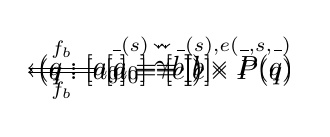
\begin{tikzpicture}[x=2.5\diagx,y=-1.5\diagy]
  \node (A) at (0,0) {$[a_0]=[b]$};
  \node (C) at (1,0) {$(q : [a_0]=[b]) \times P(q)$};
  \node (B) at (0,1) {$[a_0]=[c]$};
  \node (D) at (1,1) {$(q : [a_0]=[c]) \times P(q)$};
  \node (E) at (.5,.5) {$\gamma$};
 
  \draw[->] (A) to node [left] {$\scriptstyle{\_ \ct \glue(s)}$} (B);
  \draw[->] (A) to node [above] {$\scriptstyle{f_b}$} (C);
  \draw[->] (B) to node [below] {$\scriptstyle{f_b}$} (D);
  \draw[->] (C) to node [right] {$\scriptstyle {\_ \ct \glue(s) , e(\_,s,\_)}$} (D);
 \end{tikzpicture}
 \end{equation*}
 $\gamma$ says that this square commutes.
 Let us take some $q : [a_0]=[b]$ and see how it is mapped (using $f_1 \equiv \id$ and so on):
 \begin{equation*}
 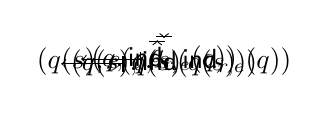
\begin{tikzpicture}[x=2.5\diagx,y=-1.5\diagy]
  \node (A) at (0,0) {$q$};
  \node (C) at (1,0) {$(q, \mathsf{ind}_{r,e}(q))$};
  \node (B) at (0,1) {$q\ct \glue(s)$};
  \node (D) at (1,1) {$(q \ct \glue(s), \mathsf{ind}(q \ct \glue(s)))$};
  \node (D2) at (1,.65) {$(q \ct \glue(s), e(q,s,\mathsf{ind}_{r,e}(q))$};
  
  \draw[|->] (A) to node {} (B);
  \draw[|->] (A) to node {} (C);
  \draw[|->] (B) to node {} (D);
  \draw[|->] (C) to node {} (D2);
 \end{tikzpicture}
 \end{equation*}
 Here, $\gamma$ tells us that the two pairs at the bottom right are equal.
 As before, we need that their second components are equal; and analogously to
 what we did before, we use $\psi^3$ to see that this is the case.
\end{proof}

\section{Equality in Pushouts}\label{sec:paths-pushout}

We already learned that pushouts and coequalizers are interderivable, so it is
an obvious question what our main theorem translates to when regarded for
pushouts instead of coequalizers.
We write $\inp: (M+N) \to \pout L M N$ for the map given by $(\inl, \inr)$.
To simplify notation, we keep the inclusions $\inl : M \to (M+N)$
and $\inl : N \to (M+N)$ implicit and only mention the inclusions into the
pushout.

Since pushouts are used a lot and play a vital role in the Seifert-van Kampen theorem 
(cf.~\Cref{sec:paths-svk}),
we want to state our main result explicitly for pushouts instead of coequalizers.
The proofs can straightforwardly be obtained by expressing the pushouts as coequalizers,
as described in the introduction. (In Lean, this is simply a specialization).

\begin{thm}[Induction for Pushout Equality] \label{thm:paths-main-pushout}
 Assume $L, M, N : \UU$, $f : L \to M$, $g : L \to N$ are given as in the
 definition of the pushout,
 together with a point $n_0 : N$.
 Assume we are given families $P, Q$ and terms $r,e$ as follows:
%  \begin{equation}
 \begin{align}
  P &: \{m : M\} \to (\inr(n_0) = \inl(m)) \to \UU \label{eq:P-mainresult-pushout}\\
  Q &: \{n : N\} \to (\inr(n_0) = \inr(n)) \to \UU \label{eq:Q-mainresult-pushout} \\
  r &: Q(\refl_{\inr(n_0)}) \label{eq:r-mainresult-pushout} \\
  e &: (l : L) \to (q: \inr(n_0) = \inl(f(l)))
       \to P(q) \simeq Q(q \ct \glue(l)). \label{eq:e-mainresult-pushout}
 \end{align}
%  \end{equation}
 Then, we can construct terms
%  \begin{equation}
 \begin{align*}
  \mathsf{ind}^P_{r,e} &: \{m : M\}(q : \inr(n_0) = \inl(m)) \to P(q) \\
  \mathsf{ind}^Q_{r,e} &: \{n : N\}(q : \inr(n_0) = \inr(n)) \to Q(q)
 \end{align*}
%  \end{equation}
 with the following $\beta$-rules:
 \begin{align*}
  \mathsf{ind}^P_{r,e} (\refl_{\inr(n_0)}) &= r \\
  \mathsf{ind}^Q_{r,e}(q \ct \glue(l)) &= e (l,q,\mathsf{ind}^P_{r,e}(q))
 \end{align*}
 \qed
\end{thm}

\begin{remark}
 As before, the first $\beta$-rule
holds judgmentally in our formalization.
\end{remark}

\begin{thm}[Initiality of Pushout Equality] \label{thm:paths-mainresult-pushout-based}
 Given the same data as in the previous theorem, we can consider the category $\CatP$,
 whose definition mirrors that of $\CatC$.
 Objects are quadruples $(J,K,r,e)$,
 \begin{align*}
  J &: M \to \UU \\
  K &: N \to \UU \\
  r &: K(n_0) \\
  e &: (l : L) \to J(f(l)) \simeq K(g(l))
 \end{align*}
and a morphism between $(J,K,r,e)$ and $(J',K',r',e')$ consists of fiberwise
functions which preserve $r$ and commute with $e$. %, $e'$.
  Then, the object $(J^i,K^i,r^i,e^i)$ defined by
 \begin{align*}
  J^i(m) &:\equiv \left(\inr(n_0) = \inl(m)\right) \\
  K^i(n) &:\equiv \left(\inr(n_0) = \inr(n)\right) \\
  r^i &:\equiv \refl_{\inr(n_0)} \\
  e^i(l) &:\equiv \_ \ct \glue(l)
 \end{align*}
is initial in $\CatP$. \qed
\end{thm}

\section{First Applications}\label{sec:paths-applications}

We anticipate that our main result, especially in the formulations of
\Cref{thm:paths-main-thm} and \Cref{thm:paths-main-pushout},
will be a very useful tool for a variety of constructions
in homotopy type theory.
In this chapter, we will present two short applications.

The \textbf{loop space} $\Omega(X)$ of a type $X$ with an (implicitly given)
point $x_0 : X$ is defined to be $x_0 = x_0$.
Thus, the loop space of the circle $\Sph^1$ is simply
$\Sbase = \Sbase$.
We can use our main result to reprove \Cref{thm:hit-s1} stating that
\begin{equation*}
\Omega(\Sone) \simeq \Z \text{.}
\end{equation*}

\begin{proof}[New proof for \Cref{thm:hit-s1}]
As discussed in \Cref{sec:coeq-hit}, $\Sone$ can be expressed as
the coequalizer of $\unit$ and
the relation which has $\unit$ as its value.
This allows us to apply \Cref{thm:paths-mainresult-cat-based} and, since all quantifications
are now quantifications over the unit type, we can safely ignore them.
Thus, $\big(\Omega(\Sone), \refl, \_ \ct \mathsf{loop}\big)$ is the initial object
in the category of pointed types with an automorphism.
Due to the uniqueness of initial objects,
all we need is that $(\Z, 0, S)$
is initial in this category.
This statement is completely removed from the higher inductive type $\Sone$;
it is a basic property of the integers, analogous to the fact that $(\N,0,S)$ 
is initial in the category of pointed types with an endofunction.
\end{proof}
Of course, the difficulty of a concrete proof for the initiality property depends
on the concrete definition of $\Z$ that one uses.
With the definition used by Licata and Shulman (essentially $\N + \unit + \N$),
this is easy albeit some work.
We will come back to definitions of the integers in \Cref{rmk:paths-generalized-squid}.

As a second application we will prove that a certain class of functions,
called embeddings, is preserved under pushouts.
\begin{defn}\label{def:paths-emb}
An \textbf{embedding} is a map $h : X \to Y$ whose fibers are propositions,
i.\,e. where, for each $y: Y$, the type
$h\inv(y) :\equiv (x:X) \times (y = h(x))$ is a proposition.
Equivalently, $h$ is an embedding if and only if 
\begin{equation} \label{eq:ap}
 \ap_h : \{x,x': X\} \to (x = x') \to (h(x) = h(x'))
\end{equation}
is a family of equivalences between path spaces.
\end{defn}

As formalized by \citet{eric:embedding-pushout} via an encode-decode construction,
embeddings are closed under pushout.
In the following, we present an alternative (and significantly shorter) argument.

\begin{thm}[Pushouts preserve Embeddings]\label{thm:paths-embedding}
 Embeddings are closed under pushout.
 Explicitly, if $f$ in following the diagram is an embedding, then so is $\inr$:
\begin{equation*}
  \begin{tikzpicture}[x=\diagx,y=-\diagy,baseline=(current bounding box.center)]
   \node (A) at (0,0) {$L$};
   \node (C) at (1,0) {$N$};
   \node (B) at (0,1) {$M$};
   \node (D) at (1,1) {$\pout L M N$};
  
   \draw[right hook->] (A) to node [left] {$\scriptstyle f$} (B);
   \draw[->] (A) to node [above] {$\scriptstyle g$} (C);
   \draw[->, dashed] (B) to node [below] {$\scriptstyle \inl$} (D);
   \draw[right hook->, dashed] (C) to node [right] {$\scriptstyle \inr$} (D);
  \end{tikzpicture}
\end{equation*}
\end{thm}

\begin{proof}
 Using \eqref{eq:ap}, we need to show that $\ap_\inr : (n_0 = n) \to (\inr(n_0) = \inr(n))$
 is an equivalence for all points $n_0, n$.
 Thus, for any $q : \inr(n_0) = \inr(n)$, we want to find something in the preimage of $q$.
 This tells us how we need to choose the type family $Q$ of \Cref{thm:paths-main-pushout}:
 We fix $n_0$ and define
 \begin{align*}
  Q &: (n : N) \to (\inr(n_0) = \inr(n)) \to \UU \\ 
  Q(n,q) &:\equiv (p : n_0 = n) \times \ap_\inr(p) = q. %%\fib_{\ap_\inr}(q).
 \end{align*}
 We also need to define the type family $P$.
 Given something in $M$, we ``move'' it back to $N$ by going via the fiber, which
 allows us to define $P$ using $Q$:
 \begin{align*}
  P &: (m : M) \to (\inr(n_0) = \inl(m)) \to \UU \\
  P(m,q) &:\equiv \left((l_0, q_0) : f^{-1}(m)\right) \times
      Q\big(g(l_0), q \ct \ap_{\inl}(q_0) \ct \glue(l_0)\big).
 \end{align*}
 The component $r$ is the obvious one,
 $r :\equiv (\refl, \refl)$.
 For a given $l:L$ we know that, since $f$ is an embedding, the type $f\inv(f(l))$
 is contractible and we can assume $(l_0, q_0) \equiv (l, \refl)$.
 This implies $P(f(l),q) \simeq Q(g(l),q \ct \glue(l))$, which is exactly what we
 need in order to define the component $e$.
 Thus, we have 
 \begin{equation*}
  \mathsf{ind}^Q_{r,e} : \{n : N\}(q : \inr(n_0) = \inr(n)) \to (p : n_0 = n) \times \ap_\inr(p) = q,
 \end{equation*}
 i.\,e. a section $s$ of $\ap_\inr$ (a function such that $\ap_\inr \circ s = \mathsf{id}$).
 To show that $s \circ \ap_\inr : (n_0 = n) \to (n_0 = n)$ is the identity,
 we do path induction and use the first $\beta$-rule.
\end{proof}

\section{Free Groupoids and a Higher Seifert-van Kampen Theorem}\label{sec:paths-svk}
\sectionmark{Free Gruopoids and Seifert-van Kampen}

Fundamental groups in topology are \emph{quotients} of spaces --
in homotopy type theory we represented them as 0-truncations of equality types.
Thus, it is natural to ask for a \emph{higher dimensional} version of the theorem
which does not quotient or truncate.
In homotopy theory, different versions have been proved by \cite{lurie18derived}
and \cite{brown2011nonabelian}.
In homotopy type theory, it is an open problem how this could be done.
The results of this chapter suggest one possible such higher Seifert-van Kampen theorem
(\Cref{thm:paths-svk}),
which we present in this section.
Note that the precise formulation of a theorem is part of the open question how
to generalize the Seifert-van Kampen theorem in homotopy type theory,
since the analogue of the $\code$ family by Favonia and Shulman has to be defined
(and a trivial solution exists: define this analogue to be the equality).
Our justification for why the analogue we suggest is reasonable is that, by
$0$-truncating, the Favonia-Shulman theorem can be recovered relatively easily.
As in \Cref{sec:paths-pushout}, let as assume $L, M, N : \UU$,
$f : L \to M$, and $g : L \to N$. We write $P :\equiv \pout{L}{M}{N}$.
A caveat is in order.
In this section, we make used of \emph{indexed higher inductive types},
of which we expect that they can be encoded in terms of higher inductive types,
analogously to the fact that indexed inductive types can always be encoded via
inductive types, as proven by \cite{indexedcontainers,Sattler:indexedW}.

To recall, the Seifert-van Kampen theorem in the version of
\cite{favonia:SvK} states that for $x, y : M + N$ there is an equivalence
\begin{equation*}
\trunc{0}{\inp(x) =_P \inp(y)} \simeq \code(x,y) \text{.}
\end{equation*}
The central difficulty of a higher version of the theorem is, of course,
avoiding the set-truncation.
Note that, in our description of the the lists used to define $\code$,
the set-truncations in 
\begin{align*}
p_i &: \trunc 0 {g(l_i) = g(k_{i+1})} \text{ and} \\
q_i &: \trunc 0 {p(k_i) = p(l_i)}
\end{align*}
can be removed since we set-truncate later
when taking the set-quotient.
This is essentially a repeated application of the equivalence
\begin{equation*}
 \trunc{n}{(a:A) \times \trunc{n}{B(a)}} \simeq \trunc{n}{(a:A) \times B(a)}.
\end{equation*}
This unnecessary set-truncation \emph{does} make sense in the formulation of the
Seifert-van Kampen theorem, where all equality types are set-truncated, but
removing it makes it easier to motivate our \emph{higher} Seifert-van Kampen theorem.

Next, we suggest an alternative definition for the type of lists (before quotienting/truncation).
To simplify things further, let us fix $n_0 : N$ and consider lists starting at this point.
Let us now look at the following \emph{indexed} inductive type $C_0 : (M+N) \to \UU$
with three constructors,
where $C_0(x)$ should be understood as a type of lists from $n_0$ to $x$.
Recall that we keep the embeddings $i_1 : M \to (M+N)$ and $i_2 : N \to (M+N)$ implicit,
and that the data we are given are maps $f : L \to M$ and $ g : L \to N$.
\begin{equation*}
\begin{gathered}
\inferrule*[left=$C_0$-Intro1]{ }{\nil : C_0(n_0)} \\[.7em]
\inferrule*[left=$C_0$-Intro2]{l : L \\ c : C_0(f(l))}{ \glconstr(l,c) : C_0(g(l))} \qquad
\inferrule*[left=$C_0$-Intro3]{l : L \\ c : C_0(g(l))}{ \glconstr'(l,c) : C_0(f(l))} \qquad
\end{gathered}
\end{equation*}
Clearly, $\nil$ gives us the empty list.
The other two constructors allow us to switch between lists ending in a point in $M$
to lists ending in a point in $N$ and vice versa.
Intuitively, this is done simply by adding a $\glue$ at the end of the list.
This explains how to add the \emph{vertical} lines of a list as drawn in \Cref{fig:hit-svk-zigzag}.
It may be surprising that we do not add the \emph{horizontal} components $p_i$ and $q_i$ explicitly.
The reason is that they are automatically and implicitly present in this encoding:
the map $(\_)^*$ of type
\begin{equation}
  \{l,l' : L\} \to (g(l) = g(l')) \to \big(C_0(g(l)) \to C_0(g(l'))\big)
\end{equation}
allows us to ``insert'' the upper horizontal components in \Cref{fig:hit-svk-zigzag}
and (exchanging $g$ by $f$) also the lower horizontal components.

The type $C_0(x)$ encodes lists from $n_0$ to $x$, but we have not done the
quotienting, i.e.\ lists that should be the same are still different.
To remedy this, we can turn $C_0$ into an indexed \emph{higher} inductive type 
and add constructors ensuring that $\glconstr(l, \glconstr'(l, x)) = x$ and
$\glconstr'(l,\glconstr(l,x)) = x$.
If we set-truncate, this would give us the correct type, namely something equivalent
to the $\code(n_0,x)$ by Favonia and Shulman. 
Since we do not want to set-truncate, we have to be more careful.
$\glconstr(l)$ and $\glconstr'(l)$ together with the equality constructors will
form a pair of \emph{quasi-inverses}~\citepalias{hottbook}, and it is known
that this type is not well-behaved.
Instead, we mirror the components that form an actual equivalence.
Although there are several formulations that would work, we use those that turn
$\glconstr$ into a \emph{bi-invertible map} ~\citepalias{hottbook}, as with
the following introduction rules for a type family $C : (M+N) \to \UU$:
\begin{equation*}
\begin{gathered}
\inferrule*[left=$C$-Intro1]{ }{\nil : C(n_0)} \qquad
\inferrule*[left=$C$-Intro2]{l : L \\ c : C(f(l))}{\glconstr(l,c) : C(g(l))} \\[.7em]
\inferrule*[left=$C$-Intro3]{l : L \\ c : C(g(l))}{\mathsf{linv}(l,c) : C(f(l))} \qquad
\inferrule*[left=$C$-Intro4]{l : L \\ c : C(g(l))}{\mathsf{rinv}(l,c) : C(f(l))} \\[.7em]
\inferrule*[left=$C$-Intro5]{l : L \\ c : C(f(l))}{\mathsf{linv}(l, \glconstr(l, x)) = x } \qquad
\inferrule*[left=$C$-Intro6]{l : L \\ c : C(g(l))}{\glconstr(l,\mathsf{rinv}(l,y)) = y}
\end{gathered}
\end{equation*}
This definition of $C$ does certainly not look very appealing, and we only give
this presentation because it is the ``standard'' way of presenting higher
inductive types.
If we allow ourselves to fold the last five constructors into a single one,
its introduction rule could look as follows:
\begin{equation*}
\inferrule*[left=$C$-Intro2--6]{l : L}{C(f(l)) \simeq C(g(l))}
\end{equation*}

It may also be interesting to do this in the formulation for a coequalizer
instead of a pushout.
As explained in \Cref{sec:paths-main}, this is a completely mechanical translation.
Thus, assume $A$ with $a_0 : A$ and $\_\sim\_$.
Then, the corresponding type $G$ in the ``folded'' form looks as follows:
\begin{equation} \label{eq:free-higher-groupoid-nice}
 \begin{alignedat}{1}
  & \mathsf{data} \; G : A \to \UU \\
   & \quad \nil : G(a_0) \\
   & \quad \cons : \{b,c:A\} \to (b \sim c) \to G(b) \simeq G(c)
 \end{alignedat}
\end{equation}
Let us write $\mathfrak G(a_0, \_)$ instead of $G(\_)$, in order to explicitly
mention the point $a_0$.
We can call $\mathfrak G$ the \emph{free higher groupoid} generated by $\sim$.
This construction generalizes the explicit construction of a free higher group
(based on an idea by \citet{kraus_FHG}).
It also generalizes the ``integer type as a higher inductive type''
(itself a special case of the free higher group) which was independently suggested
by~\citet{gun:squid} (based on Capriotti's idea),
by van der Weide et al.\ in unpublished work, and in a formalization by
~\citet{Evan:Squid}.
This example is discussed further in \Cref{rmk:paths-generalized-squid} below.

The type family $C$ depends on the chosen point $n_0$.
To remove this dependency, let us consider a version of $C$ which is indexed
twice over $(M+N)$:
we write $\mathfrak C(n_0, y)$ for $C(y)$.
This expression plays the role of $\code$ in our higher analogue of
the Favonia-Shulman result, \Cref{thm:paths-svk}.
While it can be extended to a family $P \to P \to \UU$ in a straightforward way,
we choose the following formulation for simplicity
(and to match \Cref{thm:paths-svk} more closely):

\begin{thm}[Higher Seifert-van Kampen Theorem]\label{thm:paths-higher-SvK}
 For $x,y : M+N$, we have an equivalence:
 \begin{equation} \label{eq:thm-higher-svk}
  \left(\inp(x) =_P \inp(y)\right) \simeq \mathfrak C (x,y).
 \end{equation}
\end{thm}

\begin{proof}
Like all (indexed/higher/ordinary) inductive types,
our type family $C$ is initial in an
appropriately formulated category of algebras (see \citet{awodeyGamSoja_hoAlgs},
\cite{Coquand:2018:HIT:3209108.3209197}, and others).
Here is where we draw the connection with the main result of the paper:
The category in which $C$ is initial is
the category $\CatP$ from \Cref{thm:paths-mainresult-pushout-based}.%
\footnote{To be precise, the object $(C \circ i_1, C \circ i_2, \nil, \glconstr)$ is initial in $\PP$.}
This is easy to see when we use the general specification and definition of
higher inductive-inductive types given by \citet{kaposi_et_al:LIPIcs:2018:9190,AAhiits},
but see \Cref{rmk:paths-generalized-squid} below.

By the uniqueness of the initial object and by \Cref{thm:paths-mainresult-pushout-based},
$C(x)$ is equivalent to $\inr(n_0) =_P \inp(x)$.
Letting $n_0$ vary, we get the statement of the theorem.
\end{proof}

It is relatively straightforward to recover the set-truncated SvK statement
from the higher version (\Cref{thm:paths-higher-SvK}).
We can simply set-truncate both sides in \eqref{eq:thm-higher-svk} and then prove
that $\trunc 0 {\mathfrak C(x,y)}$ is equivalent to $\code(x,y)$ by constructing
maps in both directions.

\begin{remark} \label{rmk:paths-generalized-squid}
\Cref{thm:paths-higher-SvK} and its proof 
deserve additional comments.
We think it is fair to say that the formal theory of indexed higher inductive
types is not yet well-established, but it is under very active development.
\citet{kaposi_et_al:LIPIcs:2018:9190,AAhiits} have
suggested a definition for general higher inductive-inductive types which captures
the case we need.
Indexed higher inductive types are considered in some of the cubical settings;
cf.\ \citet{cavallo2019higher}, and there are plans to extend
cubical Agda~\citep{andrea:cubicalagda,anders:cubicalblog,andreaAnders:experiments}
and redtt~\citep{redtt} with the concept (at the time of writing, a possibly not
final version is available in cubical Agda).
Our definition of $C$ would be covered by any potential implementation of
indexed higher inductive types.
We think it would be desirable to also allow a direct syntactical representation as
in
\textsc{$C$-Intro2-6}, even if only as syntactic sugar
for the rules it replaces.
Note that Kaposi and Kov{\'a}cs allow equalities between types,
which is very similar to allowing this family of equivalences.

The critical step in the above proof of \Cref{thm:paths-higher-SvK} is to establish
$C$ as the initial object of the
category $\CatP$.
With the specification suggested by Kaposi and Kov{\'a}cs allowing
\textsc{$C$-Intro2-6}, with equalities instead of
equivalences, this part is easy.
However, we want to emphasize that the initiality of
$C$ using \textsc{$C$-Intro2-6}
is not immediate at all if we use what we could call the
\emph{direct induction principle}
\footnote{The terminology was suggested by Anders M\"ortberg.}.
The direct induction principle is the ``standard'' principle one derives by
giving one case for each constructor, as done in the book~\citepalias{hottbook}
and by current proof assistants such as cubical Agda.
Unfortunately, due to the type dependency in the direct induction principle,
it becomes very hard to ``fold'' the components for the type
$C$ in order to achieve the principle one
would expect from the constructor \textsc{$C$-Intro2-6}.
We expect that implementing \Cref{thm:paths-higher-SvK} in cubical Agda would be
extremely tedious for this reason.
% (note that \Cref{thm:higher-SvK} is also not part of our Lean formalization).

The core of the problem with the direct induction principle is that it does not
allow us to ``reason on the level of constructors''.
As an example, let us consider the interval with two point constructors and one
path constructor.
If we can reason on the level of constructors, it is by ``singleton contraction''
clear that one point and the path constructor form a contractible pair, and that
the interval is therefore equivalent to the type generated by a single point.
With the direct induction principle, this style of reasoning is not possible.
It turns out to be easy enough to prove the interval contractible, but  in other
cases, the situation is less fortunate.

As an example, proposals by~\citet{gun:squid}, unpublished
work by van der Weide et al., and a formalization by Cavallo based on a remark
by M\"ortberg~\citep{Evan:Squid} suggest to define $\Z$ as a higher inductive
type, and their very definition is chosen such that $\Z$ should become the
initial object of the category of pointed types with automorphism
(cf.\ \Cref{sec:paths-applications}).
Their definitions are versions of \eqref{eq:free-higher-groupoid-nice} with
$A$ and $\sim$ replaced by the unit type and the relation constantly unit.
Crucially, they have to ``unfold'' the constructor $\cons$, since this is
what the current cubical proof assistants require.
It turns out that this makes it extremely tedious to prove the resulting
type equivalent to other definitions of the integers.
\end{remark}

\section{Formalization in Lean}\label{sec:paths-lean}

Not all, but most results of this chapter have been formalized in the
theorem prover Lean:
\begin{itemize}
\item We formalized the two wild categories $\CatC$ and $\CatD$
of \Cref{def:paths-catC} and \Cref{def:paths-catD} as structures,
\item we proved their equivalence as per \Cref{lem:paths-cats-are-iso},
\item we provided the initial element of $\CatC$ as in \Cref{lem:paths-D0-init},
\item we use it to prove the non-dependent version of the main result,
\Cref{thm:paths-mainresult-cat-based},
\item and then derive the dependent eliminator from the uniqueness of
the non-dependent one, as in the proof of \Cref{thm:paths-main-thm},
\item we specialize the result to pushouts, which in Lean, are a special case of
coequalizers,
\item we formalize the two applications of the thorem as given in
\Cref{sec:paths-applications}.
\end{itemize}
The higher Seifert-van Kampen was not formalized, since we don't have
indexed higher inductive types at our disposal in Lean.

We will now give a few code snippets as examples for how the contents
are represented in Lean.
The formalization makes heavy use of Lean's homotopy type theory library
\citep{leanhott}.

The wild categories $\CatC$ and $\CatD$ are encoded as structures, the definition
of objects and morphisms in the latter looking as follows:
\begin{leancode}
@[hott] protected structure CatD_ob :=
  (L : D → Type w')
  (n : L (ι x))

@[hott] protected structure CatD_mor (X Y : CatD_ob) :=
  (L : Π d, X.L d → Y.L d)
  (n : L _ X.n = Y.n)
\end{leancode}
Note, that \leani{@[hott]} is a user-define command which makes sure that the
strict universe of propositions is not used in any way, and thus our
formalization is indeed consistent with homotopy type theory.

The equivalence of $\CatC$ and $\CatD$ is, on objects defined and stated as
follows (we omit the proof itself here):
\begin{leancode}
@[hott] private def CatCD_ob (X : CatC_ob) : CatD_ob :=
⟨hott.quotient.elim X.K X.c, X.n⟩

@[hott] private def CatDC'_ob (X : CatD_ob) : CatC_ob :=
⟨X.L ∘ ι, X.n, λ y z r, ap X.L (eq_of_rel R r)⟩

@[hott] private def CatCD_ob_equiv : CatC_ob ≃ CatD_ob := ...

@[hott] private def CatCD_mor_equiv (X Y : CatD_ob)
  : CatD_mor X Y ≃ CatC_mor (CatDC'_ob X) (CatDC'_ob Y) := ...
\end{leancode}
The initial object of $\CatC$ is then defined by first giving the initial
object of $\CatD$ and then mapping it to $\CatC$:
\begin{leancode}
@[hott] private def CatD_init : CatD_ob := ⟨λ d, ι x = d, idp⟩
\end{leancode}

The non-dependent eliminator is manifested in the following:
\begin{leancodebr}
section elim'
parameters {Q : A → Type (max u v)}
  (x : A)
  (Qrefl : Q x)
  (Qeq : Π y z (r : R y z), Q y = Q z)
include Qrefl Qeq

@[hott] def Q_obj' : CatC_ob x := ⟨Q, Qrefl, Qeq⟩

@[hott, elab_as_eliminator] protected def path_elim' (y : A) (p : ι x = ι y)
  : Q y := ...
\end{leancodebr}

The version of the dependent eliminator for pushouts is obtained by a simple
specialization, as visble in the following snippet:
\begin{leancodebr}
section
  parameters (x : B ⊎ C)
    (Q : Π (y : B ⊎ C), ι x = ι y →  Type w')
    (Qrefl : Q x idp)
    (Qcons : Π (a : A) (p : ι x = inl (f a)), 
      Q (sum.inl (f a)) p ≃ Q (sum.inr (g a)) (p ⬝ glue a))
  include Qrefl Qcons

@[hott] private def prel : B ⊎ C → B ⊎ C → Type _ := 
@hott.pushout.pushout_rel A B C f g

@[hott] private def Qcons' (y z : B ⊎ C) (p : ι x = ι y) (r)
  : Q y p ≃ Q z (p ⬝ eq_of_rel prel r) :=
by { hinduction r with a; apply Qcons }

@[hott] protected def path_rec (y : B ⊎ C) (p : ι x = ι y) : Q y p :=
begin
  refine quotient.path_rec x Qrefl _ y p,
  exact Qcons' f g x Q Qrefl Qcons,
end
\end{leancodebr}

To emphasize the benefits of our theorem when it comes to allowing for short
proofs of homotopy theoretic statements,
let us look at the proof of the theorem stating that pushouts preserve embeddings
(\Cref{thm:paths-embedding}) in full:
\begin{leancodebr}
parameters {A : Type u} {B : Type v} {C : Type w} (f : A → B) (g : A → C)
  [is_embedding f]
include f g

@[hott] def motive {c₀} :
  Π x (q : (inr c₀ : pushout f g) = quotient.class_of _ x), Type _
| (sum.inl b) q := Σ (a : fiber f b),
                     fiber (ap inr) (q ⬝ ap inl a.2⁻¹ ⬝ (glue a.1))
| (sum.inr c) q := fiber (ap inr) q

@[hott] def fib_rec (c₀ c q) : @motive c₀ (sum.inr c) q :=
let Qcons : Π a (p : inr c₀ = inl (f a)), 
            motive (sum.inl (f a)) p ≃ motive (sum.inr (g a)) (p ⬝ glue a) :=
 λ a p, @sigma_equiv_of_is_contr_left _
    (λ (a : fiber f (f a)), fiber (ap inr) (p ⬝ ap inl (a.2)⁻¹ ⬝ glue (a.1))) 
    (is_contr_of_inhabited_prop ⟨a, idp⟩) in
pushout.path_rec f g _ motive ⟨idp, idp⟩ Qcons _ q

@[hott] protected def preserves_embedding : is_embedding inr :=
λ c c', adjointify _ (λ q, (fib_rec c c' q).1)
  (λ p, (fib_rec c c' p).2) (λ p, by { hinduction p, refl })

\end{leancodebr}


%TODO
% give example structures for the categories
% give statement of the main thm
% give proof of embedding lemma, accent its brevity




